\section{Задача H. Отчёт об ошибках}

\begin{frame}[t]{Задача H. Отчёт об ошибках}

  \begin{center}
    \LARGE Задача H. Отчёт об ошибках
  \end{center}
  \begin{center}
	  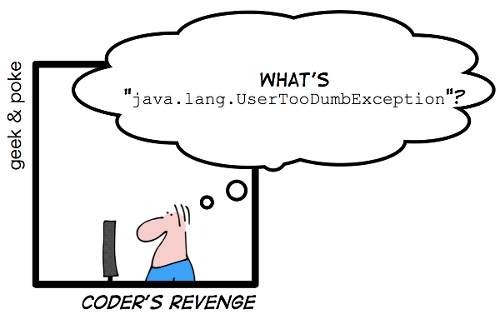
\includegraphics[width=7cm]{pics/log.png}
  \end{center}
\end{frame}

\begin{frame}[t]{}
  \vspace{3cm}
  \begin{itemize}
    \item Идея задачи --- Юрий Петров
    \item Подготовка тестов --- Николай Будин
    \item Разбор задачи --- Николай Будин
  \end{itemize}
\end{frame}

\subsection{Постановка задачи}

\begin{frame}[t]{Постановка задачи}
\begin{itemize}
    \item Дана распечатка стека вызовов.
    \item Нужно найти программу с минимальной возможной сложностью, способную сгенерировать такую распечатку.
\end{itemize}
\end{frame}

\subsection{Решение задачи}

\begin{frame}[t]{Решение задачи}
\begin{itemize}
    \item Заметим, что функция, стоящая на первом месте в распечатке обязательно должна содержать в себе ошибку.
    \item Пусть мы зафиксировали вторую функцию, в которой происходит ошибка.
    \item Тогда посмотрим на все пары последовательных функций, присутствующие в распечатке.
    \item Если функция, из которой происходит вызов, может упасть из-за ошибки, не будем учитывать эту пару.
    \item Тогда количество учтённых уникальных пар, является ответом.
\end{itemize}
\end{frame}

\begin{frame}[t]{Решение задачи}
\begin{itemize}
    \item Для каждой функции предподсчитаем количество различных функций, вызываемых из нее в распечатке.
    \item Тогда, при паре зафиксированных функций с ошибками, ответом является общее количество уникальных пар минус предподсчитанные значения для функций с ошибками.
    \item Переберем вторую функцию с ошибкой и выберем ту, при которой ответ минимален.
\end{itemize}
\end{frame}
